\chapter{Iterative design}
\section{Complementary Optimization in 1D}
\subsection{Motivation for a Complementary Optimization Strategy}
The fundamental problem in the previous examples is actually not in the methods themselves, but in the improper selection of a target field. In fact, it is very difficult to select a suitable target resonant field because not every resonant mode even has a corresponding dielectric structure that is able to reproduce it. Furthermore, it is nearly impossible to select a multi-dimensional field which corresponds to a well-behaved, isotropic and discretely-valued $\epsilon$, as would be needed for practical structures. 

For this reason, a successful method must be allowed to either modify the target field, or specify it completely, in which case the user would only determine certain characteristics (e.g. mode-volume, Q-factor) that the target field should have. The former strategy is developed in both one and two dimensions, while the latter strategy is implemented in Section \ref{sec:2Dbounded} in order to design two-dimensional resonators with discrete values of $\epsilon$.

\subsection{Complementary Optimization}\label{sec:comp}
We start with the same target field as in the previous examples but we now formulate a method that allows for it to be modified during the design process. The formulation chosen is a complementary optimization routine, where we continually alternate between modifying $\epsilon$ to better fit the field, and then modifying the field to better fit $\epsilon$. Here, we use the term ``fit'' to mean that either $\epsilon$ or $H$ is solved so that the residual error from eq.~\eqref{trad ev} is minimized. Additionally, both iterations are regularized in order to stably approach a solution. This algorithm can be summarized as follows, 
\begin{align}
&\text{choose $x_0$ and $y_0$} \nonumber \\
&\text{for } i = 1, 2, \ldots \nonumber \\
&\quad\minimize_{y_i}\quad \|B_{i-1} y_i-d_{i-1}\|^2 + \eta_1\|y_i-y_{i-1}\|^2 \label{comp1}\\
&\quad\minimize_{x_i}\quad \|A Y_i A x_i - \xi x_{i-1}\|^2 + \eta_2\|x_i-x_{i-1}\|^2 \label{comp2}
\end{align}
where $Y_i = \text{diag}(y_i)$, $B_i = A \cdot \text{diag}(A x_i)$ and $d_i = \xi x_i$. $\|A Y_i A x_i - \xi x_{i-1}\|^2$ is used instead of $\|A Y_i A x_i - \xi x_{i}\|^2$ to avoid the trivial $x_i = 0$ solution and does not affect the overall accuracy since $x$ changes very slowly. 

\begin{figure}[htbp]\centering
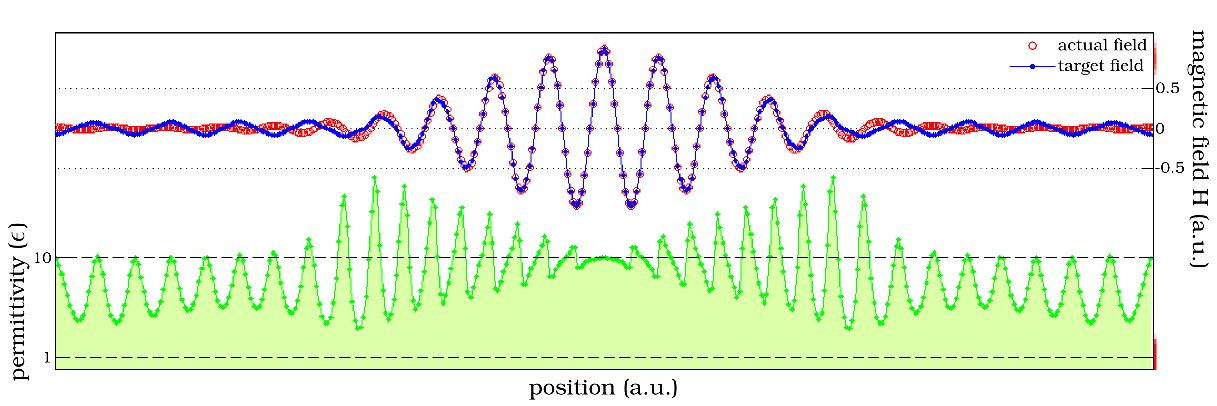
\includegraphics[width=\textwidth]{p1/complementary}
\caption{Inverse design of a one-dimensional structure using the complementary optimization method. The target field in Figs \ref{ls pic} and \ref{regls pic} is used as the initial target field. The rates of change for both $\epsilon$ and $H$ are controlled by regularization parameters $\eta_1=10^{-4}$ and $\eta_2=10^{-3}$ respectively. The $400$ iterations used to achieve this result took $60$ seconds to compute. This method results in a well-behaved $\epsilon$ that actually produces a field very similar to the original target field. Interestingly, the formation of a ``steady-state'' periodic structure toward the sides of the structure has emerged.}
\label{comp pic}
\end{figure}

Fig.~\ref{comp pic} shows that the complementary optimization algorithm, after $400$ iterations and with the correct choice of regularization parameters $\eta_1$ and $\eta_2$, results in a well-behaved structure that is able to closely reproduce the modified target field. Numerically, the least-squares problem must now be solved numerous times, which increases the computational time needed to around $60$ seconds. 

\subsection{Complementary Optimization with Bounded $\epsilon$}
In order to achieve a more practical, discretely-valued dielectric structure, we can impose strict upper- and lower-bounds on $\epsilon$. To this end, we modify our algorithm as such,
\begin{align}
&\text{choose $x_0$ and $y_0$} \nonumber \\
&\text{for } i = 1, 2, \ldots \nonumber \\
&\quad\minimize_{y_i}\quad \|B_{i-1} y_i-d_{i-1}\|^2 \nonumber \\
&\quad\text{subject to}\quad \epsilon_\text{max}^{-1} \leq y_i \leq \epsilon_\text{min}^{-1} \label{bc1} \\
\nonumber \\
&\quad\minimize_{x_i}\quad \|A Y_i A x_i - \xi x_{i-1}\|^2 + \eta_2\|x_i-x_{i-1}\|^2. \label{bc2}
\end{align}
In this algorithm, eq.~\eqref{bc1} is a convex optimization problem\cite{BV04}. This allows us to impose hard constraints on $\epsilon$, which in turn allows us to remove the regularization term present in eq.~\eqref{comp1}. The \emph{CVX} package\cite{CVX}, a Matlab-based modeling system for convex optimization, is used to solve eq.~\eqref{bc1}, with each iteration of the algorithm now requiring roughly $1$ second of computation time.
\begin{figure}[htbp]\centering
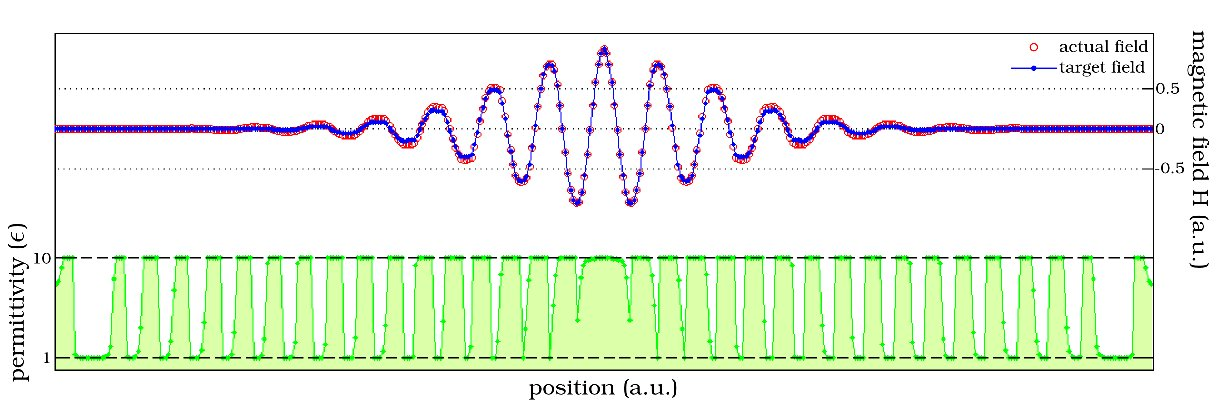
\includegraphics[width=\textwidth]{p1/bounded}
\caption{Inverse design of a one-dimensional structure using the complementary optimization method with bounded $\epsilon$. The parameters are identical to those used to produce Fig.~\ref{comp pic} with the exception that only one regularization term is now needed ($\eta_2=10^{-3}$). The algorithm was run for $100$ iterations, which took $100$ seconds. The structure turns out to be almost completely binary-valued and looks like a periodic structure with tapered duty cycle. It produces an actual field which very closely matches the final target field.}
\label{bounded comp pic}
\end{figure}

A nearly binary-valued dielectric structure is obtained in Fig.~\ref{bounded comp pic}, which accurately produces the final target field. This is very useful for the design of practical structures, since they usually consist of two or three different materials at most. Interestingly, although the directly discreteness of $\epsilon$ was not enforced (since that would make the problem non-convex), a discrete, binary-valued structure has still arisen. 

\section{Complementary Optimization in 2D}
\subsection{``S'' Resonator}
We now demonstrate that the complementary optimization method is versatile and can be scaled to multiple dimensions. To ensure that $\epsilon$ is well-behaved we use a point-spread function which does not allow $\epsilon$ to change at a certain point in space without affecting the values surrounding it. 

In order to show that our method can produce complex designs, we choose an S-shaped target field which is non-trivial to reproduce. The optimization results, using the complementary optimization method from Section \ref{sec:comp}, are shown in Fig.~\ref{S pic}. The resulting dielectric structure is continuous, unbounded and contains some singularities (white dots), but the final target and actual fields match up well. Also, the computational cost remains quite reasonable; the $50$ iterations needed required only $5$ minutes of computation time. The resulting structure is completely unintuitive, and illustrates the kind of new capabilities offered by the inverse design strategy. Specifically, that a complex, intricate structure can be designed just by specifying the shape and frequency of a rather simple electromagnetic mode.
\begin{figure}\centering
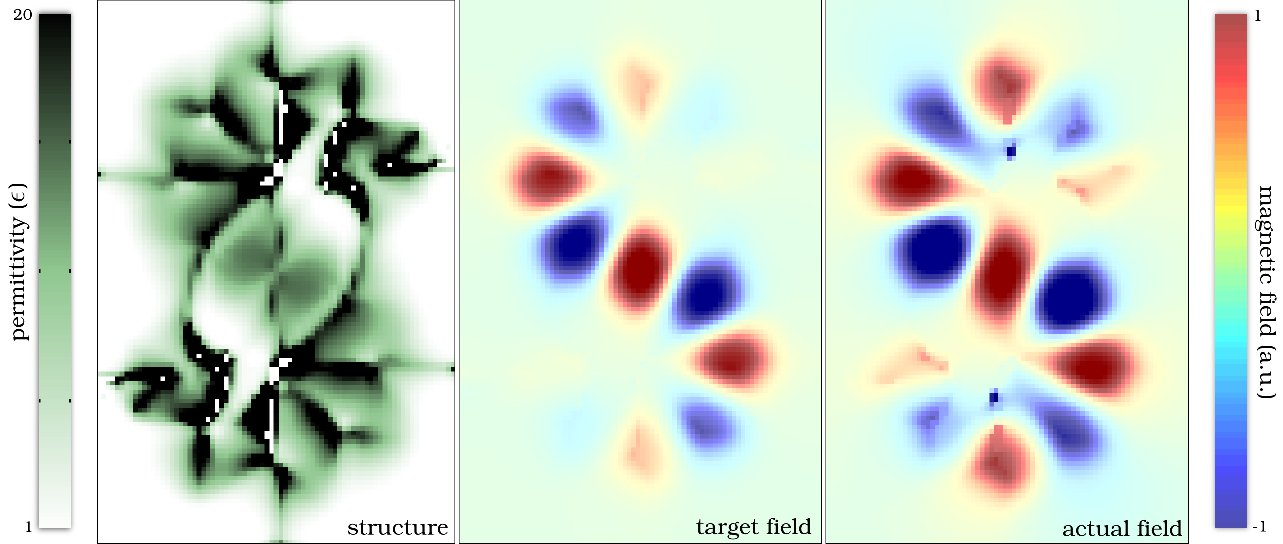
\includegraphics[width=\textwidth]{p1/S}
\caption{Inverse design of an ``S'' resonator using the complementary optimization method without bounds on $\epsilon$. The design was initialized by specifying an initial dielectric structure ($\epsilon=1$ everywhere) and a resonant field in the shape of an ``S''. The final dielectric structure was produced after $50$ iterations which took $90$ seconds to complete in total. The grid size was $80\times 120$. The final dielectric structure is quite unintuive, and yet reproduces the target field surprisingly well. This example demonstrates the versatility of the complementary optimization method in producing designs, from very simple specifications, which otherwise could be attained only with considerable difficulty.}
\label{S pic}
\end{figure}

\subsection{Multi-Mode Inverse Design}
The complementary optimization method can also be extended to produce dielectric structures with multiple resonances. To do so, multiple initial target fields are specified. The dielectric structure is first modified to simultaneously fit all target fields using a multi-objective least-squares method. Then each target field is individually modified to fit the structure; and we continue alternating between optimizing $\epsilon$ and $H^{(j)}$ in this way. A benefit of this scheme is that only the $\epsilon$ optimization increases in size, so the design process remains computationally tractable, even for several resonant fields. This algorithm can be summarized as follows,
\begin{align}
&\text{choose $y_0$, $x^{(1)}_0$, $x^{(2)}_0$, \ldots} \nonumber \\
&\text{for } i = 1, 2, \ldots \nonumber \\
&\quad\minimize_{y_i}\quad \eta_1\|y_i-y_{i-1}\|^2 + \sum_j \|B^{(j)}_{i-1} y_i-d^{(j)}_{i-1}\|^2  \label{mm1}\\
&\quad\text{for } j = 1, 2, \ldots \nonumber \\
&\quad\quad\minimize_{x^{(j)}_i}\quad \|A Y_i A x^{(j)}_i - \xi x^{(j)}_{i-1}\|^2 + \eta_2\|x^{(j)}_i-x^{(j)}_{i-1}\|^2. \label{mm2}
\end{align}
The design of an ``X'' resonator with two perpendicular, degenerate modes is shown in Fig.~\ref{X pic}. The added complexity increases the total computation time to $5$ minutes for $40$ iterations of the algorithm. 
\begin{figure}\centering
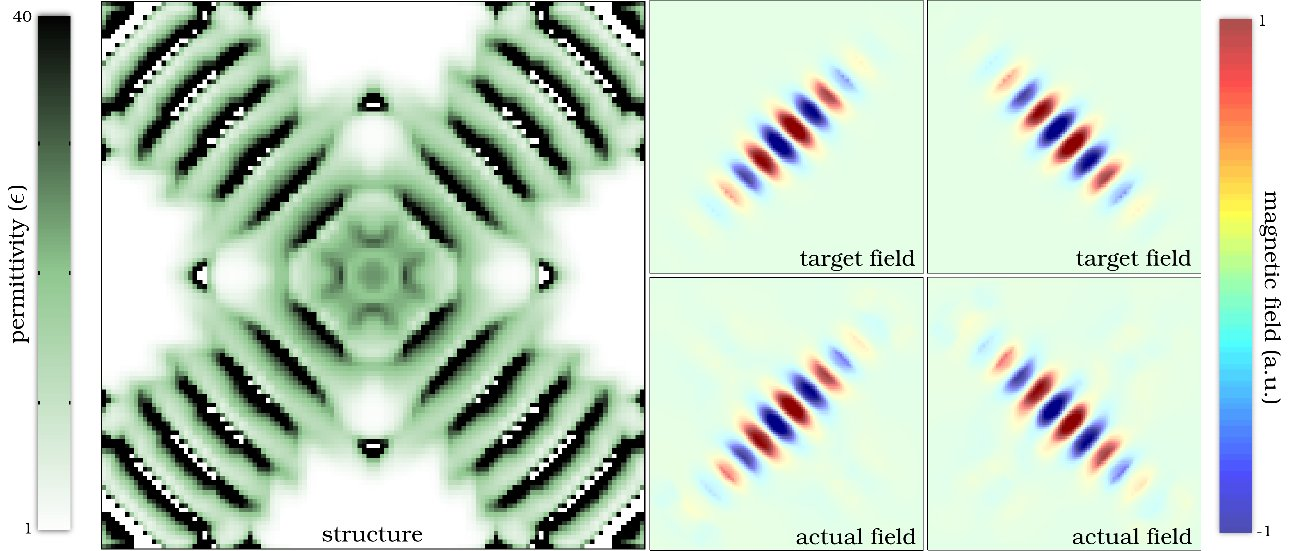
\includegraphics[width=\textwidth]{p1/X}
\caption{Inverse design of a doubly-resonant, degenerate ``X'' resonator produced by the complementary optimization method with unbounded $\epsilon$. As in Fig.~\ref{S pic} the initial value of $\epsilon$ was $1$ everywhere. The two initial target fields used are only slightly perturbed and are very similar to the two final actual target fields. Computationally, this design took $5$ minutes to complete on a $120\times 120$ grid and required $40$ iterations. This example shows that the complementary optimization strategy can be extended to produce dielectric structures with multiple resonances. Such an ``X'' resonator is useful for polarization-entangled single-photon sources for example\cite{Hen06}.}
\label{X pic}
\end{figure}

\subsection{Design of Waveguiding Devices}
The multi-mode inverse design method can also be applied to the design of waveguiding devices such as multiplexers/demultiplexers, waveguide couplers, crossbars and dispersion-tailored waveguides. This can be accomplished by treating a waveguiding device as a doubly-degenerate resonator at its operational frequencies and then enforcing opposite symmetries (even/odd or cosine/sine) in the degenerate modes. A single-to-dual beam waveguide coupler designed based on Eq.~\eqref{mm1} and \eqref{mm2} is shown in Fig.~\ref{wg pic}, and motivates how one might design other waveguiding devices such as channel-drop filters. 
\begin{figure}[htbp]\centering
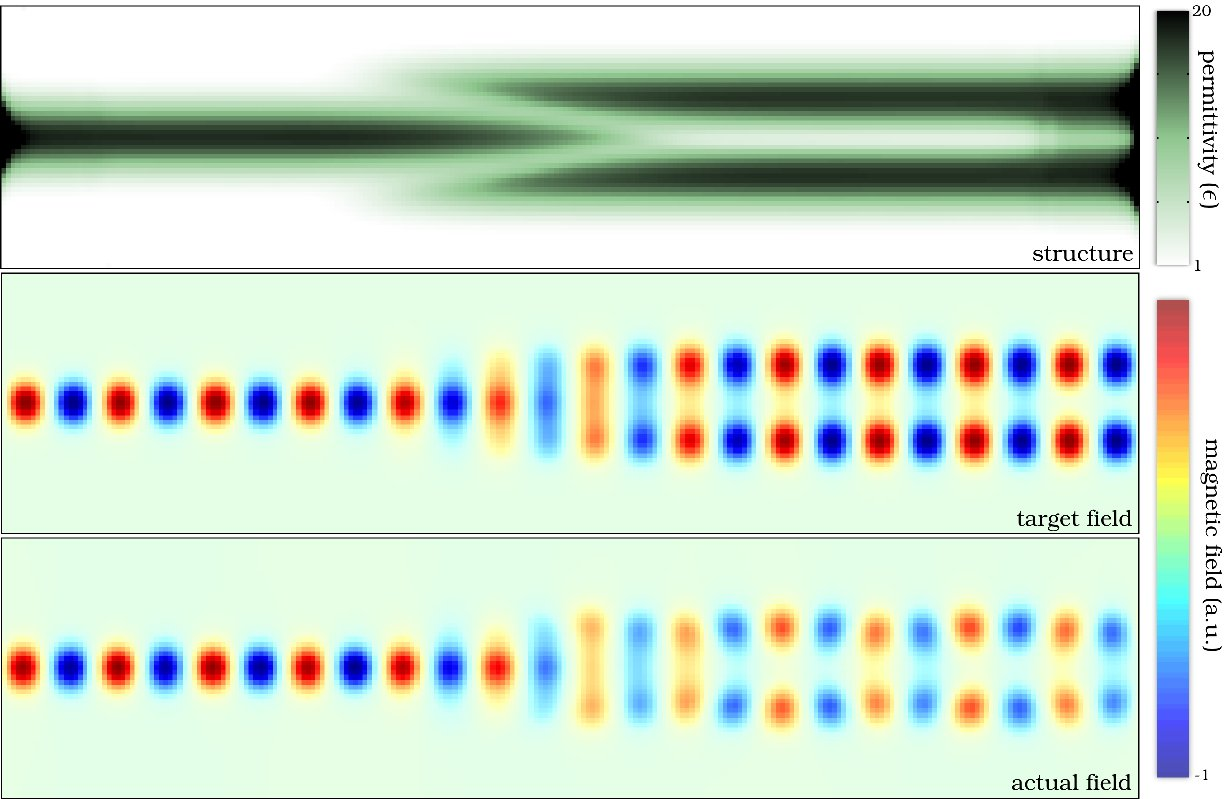
\includegraphics[width=\textwidth]{p1/wg}
\caption{Inverse design of a single-to-dual beam waveguide coupler using the complementary optimization method without bounds on $\epsilon$. Two degenerate modes with opposite symmetry (sine and cosine) are used as target fields. Only $4$ iterations ($14$ seconds) are needed to achieve this solution on a $240\times 55$ grid. This is a simple demonstration showing that the complementary optimization method can also be extended to design waveguiding devices.}
\label{wg pic}
\end{figure}
In addition to macroscopic waveguiding devices, one should also be able to create novel periodic waveguiding structures. For instance, by controlling the frequency of a particular waveguiding mode at each of its $k$-vectors, one could create a waveguide with a customized dispersion characteristic, which would be useful in the design of slow-light waveguides.


\section{Complementary Optimization with Bounded $\epsilon$ in 2D}\label{sec:2Dbounded}
\subsection{Numerical Method}\label{sec:2Dnum}
We now use the complementary optimization method to design resonators with discrete, binary $\epsilon$ in two dimensions. At the same time, the algorithm is modified so that we no longer specify an initial target field; instead, only an initial dielectric structure and the maximum desired mode volume (i.e. mode area in 2D) are specified. In addition, the optimization process attempts to maximize the Q-factor. Such an algorithm now consists of iteratively solving two convex optimization problems,
\begin{align}
&\text{choose $y_0$} \nonumber \\
&\text{for } i = 1, 2, \ldots \nonumber \\
&\quad\minimize_{x_i}\quad \|A Y_{i-1} A x_i - \xi x_{i}\|^2 +   \eta \|F x_i\|^2\nonumber \\
&\quad\text{subject to}\quad (A x_i)^T Y_{i-1} (A x_i) \leq A_\text{mode} \label{be1} \\
\nonumber \\
&\quad\minimize_{y_i}\quad \|B_i y_i-d_i\|^2 \nonumber \\
&\quad\text{subject to}\quad \epsilon_\text{max}^{-1} \leq y_i \leq \epsilon_\text{min}^{-1}. \label{be2} 
\end{align}
In this algorithm, the field optimization, Eq.~\eqref{be1}, differs significantly from Eq.~\eqref{bc2}. First, the eigenvalue equation term $\|A Y_{i-1} A x_i - \xi x_{i}\|^2$ no longer utilizes $x_{i-1}$. Also, a new ``Fourier-minimizing'' term $\|F x_i\|^2$ has been added. Here, the row vectors of $F$ consist of the field Fourier components that we do not want incorporated in the final solution. The motivation for adding this term is to design high-Q resonators using planar structures, where the Q-factor is limited by out-of-plane losses, and can thus be improved by eliminating field Fourier components that are not localized by total internal reflection (components inside the light cone)~\cite{Vuc05}. Lastly, the $(A x_i)^T Y_{i-1} (A x_i)$ term allows us to specify the mode area (mode volume in three dimensions), that we desire for our resonant field. This works because the two minimization objectives in Eq.~\eqref{be1} will generally cause the mode area to be as large as possible, which means we always end up with $(A_1 x_i)^T Y_{i-1} (A_1 x_i) = A_\text{mode}$.

The addition of the two new terms in Eq.~\eqref{be1} signifies that the field iteration in our algorithm attempts to do more than to just satisfy Maxwell's equations. Rather than only trying to fit the dielectric structure, the resonant field now also minimizes some of its Fourier components while working with a limited mode area. 

In contrast with the field optimization given by Eq.~\eqref{be1}, the structure optimization given by Eq.~\eqref{be2} remains identical to the equation in the one-dimensional case, Eq.~\eqref{bc1}, and contains no terms related to notions of Fourier components or mode area. In fact, the only objective in the $\epsilon$ optimization is to better fit the field generated from the field optimization. This means that in this scheme, the field iteration is leading the structure iteration. In other words, Eq.~\eqref{be1} ``looks ahead'' and gradually adapts itself to become a more desirable field, while Eq.~\eqref{be2} just ``follows along''. For this reason, this algorithm is unique from the other complementary optimization algorithms previously presented in the article, since in those algorithms both iterations follow one another and eventually ``meet in the middle''.

Finally, in this scheme, we chose to limit the degrees of freedom of both $x_i$ and $y_i$. Some components of $x_i$ were fixed at non-zero values and were not allowed to be modified simply to avoid the $x_i = 0$ situation. To enhance the aesthetics of the resulting dielectric structure, some components of $y_i$ were frozen as well, which is useful in cases where one would only like to modify the dielectric structure within a waveguide only, for example. 

\subsection{Circular Grating Resonator}
\begin{figure}[htbp]\centering
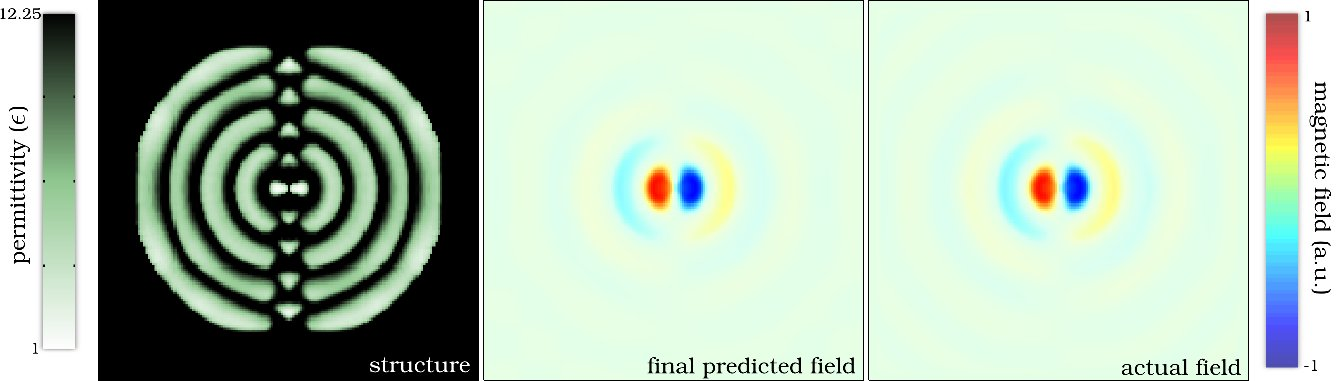
\includegraphics[width=\textwidth]{p1/circle}
\caption{Inverse design of a two-dimensional resonator using the complementary optimization method with strict bounds on $\epsilon$. The initial specification is very simple and consists an initial dielectric structure ($\epsilon=12.25$ everywhere), the frequency and mode-volume of the resonance field as well as a weighting factor, $\eta$, to avoid leaky field Fourier components. Additionally, the values of $\epsilon$ are only allowed to be modified within a central circular region and must be kept between $1$ and $12.25$. After $40$ iterations on a $160 \times 160$ grid, which took $7$ minutes to complete, a discrete structure emerged with excellent match between the predicted ($x_{40}$) and actual fields. The structure resembles a circular grating with a bowtie-like central structure for focusing the resonant energy to a single point.} 
\label{circle pic}
\end{figure}
Fig.~\ref{circle pic} shows the design of a circular grating resonator using the method from Section \ref{sec:2Dnum}. The dielectric structure emerged from a very simple choice of initial structure, namely a constant $\epsilon=12.25$ everywhere. The range of $\epsilon$ was limited to be from $1$ to $12.25$, the mode area was set to $5$ and $\eta= 10^{-3}$. Central components of $x_i$ were held constant to ensure that an electric dipole in the y-direction was produced in the center of the structure. Additionally, the components of $\epsilon$ outside a specified circle were held at a constant $\epsilon=12.25$ for the duration of the design process. The entire algorithm was run for $40$ iterations and took $7$ minutes.

After $40$ iterations, we see that a strong binary-valued structure has formed. Interestingly, the central bowtie-like structure has emerged from previous geneetic optimization methods as well\cite{Lip08}. Note also the extremely small amount of information needed to produce this result: only the frequency and mode area of the resonant field desired, and a trivial intial $\epsilon$. The ability to produce a rather advanced design from such a simple problem specification highlights the potential usefulness of inverse methods in the design of novel nanophotonic devices.

\subsection{Beam Resonator}
The same approach was used to design a beam resonator as shown in Fig.~\ref{line pic}. The parameters used in this design are identical to those used for the circular resonator, with the exception that the initial dielectric structure now consists of an unbroken waveguide, and the region where $\epsilon$ can be modified is now confined to the center of the waveguide.
\begin{figure}[htbp]\centering
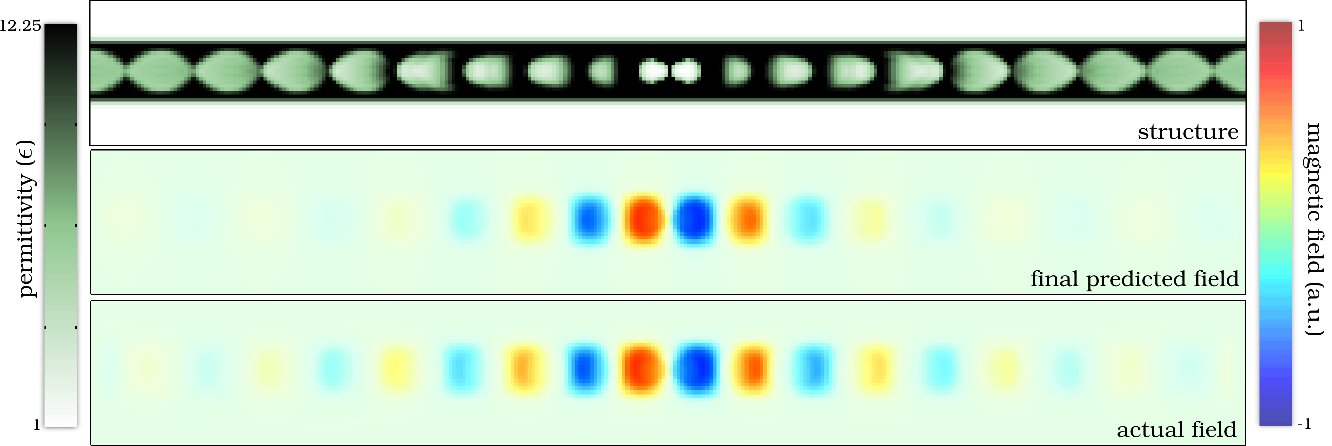
\includegraphics[width=\textwidth]{p1/beam}
\caption{Inverse design of a beam resonator in two dimensions using the complementary optimization method with bounded $\epsilon$. The initial conditions are identical to those for Fig.~\ref{circle pic}, except that the initial dielectric structure is an unbroken waveguide, and $\epsilon$ can only be modified within that waveguide. The structure emerged after $40$ iterations on a $320\times 40$ grid, which took $5$ minutes of computation. The bowtie-like structure has reappeared in the center. Interestingly, the effect of the Fourier term in Eq.~\eqref{be1}, is seen in the outward tapering of the holes.}
\label{line pic}
\end{figure}

These two, simple modifications produce a vastly different result as is plainly seen from Fig.~\ref{line pic}. Some characteristics remain, such as the two closely spaced holes in the center of the structures which focus the electromagnetic energy to a central point. Other features are unique to the beam resonator, such as a gradual outward tapering of hole diameters and size ending in a periodic ``steady-state'' structure, in similar fashion to Fig.~\ref{comp pic}. This tapering is a direct result of the Fourier term in Eq.~\eqref{be1} as it leads to a smooth field profile variation and minimization of the components in the light cone that lead to out-of-plane losses\cite{Vuc05,Aka05}.

\section{Conclusions and Outlook}
In summary, we have introduced and demonstrated a complementary optimization method for the inverse design of nanophotonic resonators as well as waveguiding structures. We have demonstrated that, in two dimensions, this method can be used to design non-trivial as well as multi-resonant structures. Furthermore, we have shown that by constraining the range of available dielectric constants, the same underlying method can produce binary-valued, discrete dielectric structures. 

The methods presented here can readily be extended into three dimensions. In essence, the only hurdle is the size of the convex optimization problem for the field optimization. Since a full three-dimensional grid often consists of tens of millions of variables, solving the field optimization problem, Eq.~\eqref{be1}, using methods such as LU factorization is no longer computationally tractable. Instead, iterative methods such as truncated Newton methods must be employed. As it turns out, such iterative methods are especially well suited to this complementary optimization scheme, since they can take advantage of the information in $x_{i-1}$ in order to solve $x_i$ very quickly. This is very applicable to our algorithm since the field changes very little from one iteration to the next. 

Although solving the field optimization problem is numerically challenging in three dimensions, solving the structure optimization problem, Eq.~\eqref{be2}, in three dimensions is much simpler. This is because only structural variations in-plane need to be accounted for planar nanophotonic devices. The number of variables in Eq.~\eqref{be2} for both two- and three-dimensional problems is then effectively the same, and the same numerical techniques can be employed to solve both.

A full three-dimensional inverse design method based on complementary optimization would enable the design of novel nanophotonic resonators. For instance, a resonator for efficient wavelength-conversion could be designed by creating a structure with multiple well-placed resonant frequencies~\cite{Riv09}. Furthermore, effects such as mode overlap and the use of frequency-dependent refractive index materials could be taken into account with such a method. 


\subsection*{Acknowledgements}
This work has been supported in part by the AFOSR MURI for Compex and Robust On-chip Nanophotonics (Dr. Gernot Pomrenke).
We thank Prof. Stephen Boyd for many fruitful discussions regarding convex optimization.

% 
% \documentclass[10pt,letterpaper]{article}
% \usepackage{opex3}
% \usepackage{amsmath}
% \usepackage{graphicx}
% 
% \begin{document}
% \title{Inverse design of a three-dimensional nanophotonic resonator}
% \author{Jesse Lu, Stephen Boyd, and Jelena Vu\v{c}kovi\'{c}}
% \address{Stanford University, \\ Stanford, C.A., 94305}
% \email{jesselu@stanford.edu}
% 
% 
% \begin{abstract} 
% The inverse design of a three-dimensional nanophotonic resonator is presented. The design methodology is computationally fast (10 minutes on a standard desktop workstation) and utilizes a 2.5-dimensional approximation of the full three-dimensional structure. As an example, we employ the proposed method to design a resonator which exhibits a mode volume of $0.32(\lambda/n)^3$ and a quality factor of $7063$. % 8808 35648
% \end{abstract}
% 
% \ocis{(230.5750) Resonators.} % REPLACE WITH CORRECT OCIS CODES FOR YOUR ARTICLE
% 
% %%%%%%%%%%%%%%%%%%%%%%% References %%%%%%%%%%%%%%%%%%%%%%%%%
% \begin{thebibliography}{99}
% \bibitem{miller} D. A. B. Miller, ``Rationale and challenges for optical interconnects to electronic chips,'' Proc. of the IEEE \textbf{88}, 728-749 (2000).
% \bibitem{prevwork} J. Lu and J. Vuckovic, ``Inverse design of nanophotonic structures using complementary convex optimization,'' Opt. Express \textbf{18}, 3793-3804 (2010).
% \bibitem{inan} U. Inan, A. Inan, \emph{Electromagnetic Waves} (Prentice Hall, 2000), page 296.
% \bibitem{yee} K. Yee, ``Numerical solution of initial boundary value problems involving maxwell's equations in isotropic media,'' IEEE Trans. Antennas Propag. Mag. \textbf{14}, 302-307 (1966).
% \bibitem{boydbook} S. Boyd and L. Vandenberghe, \emph{Convex Optimization} (Cambridge University Press, 2004).
% \bibitem{altdir} S. Boyd, N. Parikh, E. Chu, B. Peleato, and J. Eckstein are preparing a manuscript to be called, ``Distributed Optimization and Statistical Learning via the Alternating Direction Method of Multipliers,'' \verb+http://www.stanford.edu/~boyd/papers/distr_opt_stat_learning_admm.html+. 
% \bibitem{cholmod} Y. Chen, T. A. Davis, W. W. Hager, and S. Rajamanickam, ``Algorithm 887: CHOLMOD, supernodal sparse Cholesky factorization and update/downdate,'' ACM Trans. Math. Software \textbf{35}, No. 3, 2009.
% \bibitem{cvx} M. Grant and S. Boyd, \emph{CVX: Matlab software for disciplined convex programming}, version 1.21. \verb+http://cvxr.com/cvx+, January 2011.
% \bibitem{digitize} D. Englund, I. Fushman, and J. Vuckovic, ``General recipe for designing photonic crystal cavities,'' Opt. Express \textbf{13}, 5961-5975 (2005).
% \end{thebibliography}
%  
% %%%%%%%%%%%%%%%%%%%%%%%%%%  body  %%%%%%%%%%%%%%%%%%%%%%%%%%
\section{Begin of 2.5 D (Motivation)}
To date, the design of nanophotonic devices has generally involved a lengthy (days, weeks) process in which one perturbs, by trial-and-error, canonical structures such as photonic crystals or waveguide-coupled rings to achieve the desired performance for the device. 

Instead, an inverse design method in which the user only specifies the desired electromagnetic field, or characteristics thereof, and then leaves the computer to find a dielectric structure satisfying these requirements, would be a much more intuitive and computationally efficient design strategy. Furthermore, such a method may even be the only feasible option available for the design of more complex multi-wavelength and multi-functional nanophotonic devices needed for on-chip integration\cite{miller}.

\section{2.5-dimensional approximation}
Previously, we demonstrated the inverse design of various nanophotonic devices in two dimensions\cite{prevwork}.
Unfortunately, to directly extend our previous method to full three-dimensional space requires solving for a very large ($\sim 10^7 \times 10^7$) and ill-conditioned matrix, namely that given by the time-harmonic Maxwell's equation in three dimensions, which for the electric ($E$) field is
\begin{align}
\nabla\times\nabla\times E - \mu\omega^2\epsilon E &= 0,\quad\text{where}\label{wave} \\
E &= E(x,y,z).
\end{align}

Therefore, to make our problem more tractable, we formulate a 2.5-dimensional approximation of the electromagnetic fields of a planar three-dimensional nanophotonic device. As shown in Fig.~\ref{approx}a, this involves treating a planar three-dimensional nanophotonic device as a truncated holey fiber with identical dielectric structure. We take advantage of the planar nature of most nanophotonic devices in this way to produce a tractable, computationally-fast method. The $E$-field inside such a holey fiber is expressed as
\begin{equation}
E = E(x,y)e^{-i\beta z},
\end{equation}
where $\beta$ is the wave-vector along the fiber axis. Solving for Eq.~\ref{wave} now requires solving for a much smaller ($\sim 10^5 \times 10^5$) matrix, which can be accomplished using standard linear algebra packages. This simulation technique is thus very similar to a two-dimensional finite-difference frequency-domain solve.

As an example, in Fig.~\ref{approx}b, we compare the 2.5-dimensional electric field against the three-dimensional simulated electric field (at the central plane of the slab), given by a standard finite-difference time-domain (FDTD) software package, for an L3 photonic crystal resonator. We see that with the appropriate choice of $\beta$, which we obtain by fitting a sinusoid to the out-of-plane decay in the three-dimensional FDTD solution, our approximation captures most of the characteristics of the three-dimensional field at the center plane of the slab. 
\begin{figure}[hbt]
\centering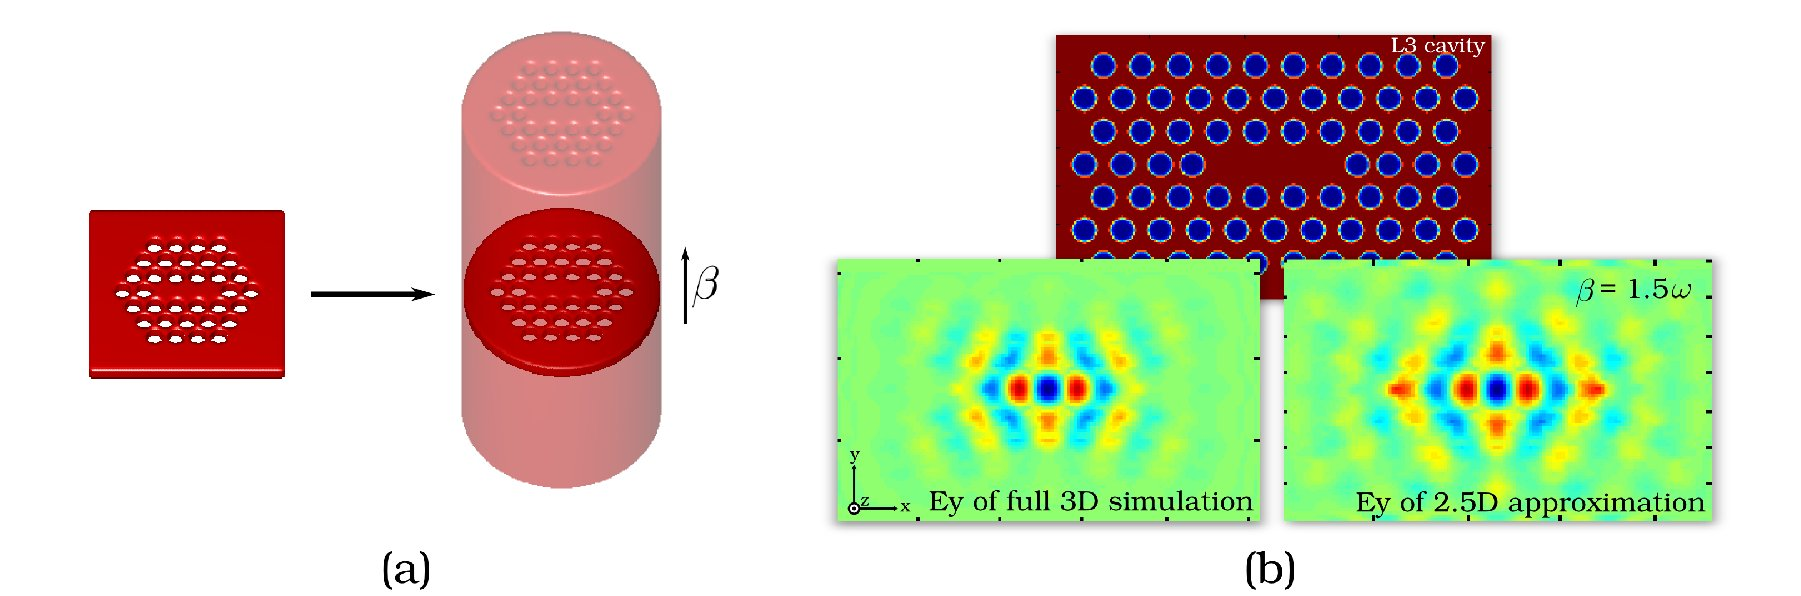
\includegraphics[width=\textwidth]{p2/approx}
\caption{(a) For computational feasibility, the resonant fields of a planar nanophotonic device are approximated as those of a truncated holey fiber with identical dielectric structure. (b) An example of our approximation using an L3 photonic crystal resonator. Most of the characteristics of the full three-dimensional field at the center of the slab appear in the approximate solution.}\label{approx}
\end{figure}

In this approximation, converting from a 2.5-dimensional structure to a full three-dimensional structure only requires the correct choice of slab thickness, $t$, since the in-plane values of $\epsilon$ remain the same. To estimate $t$ for the full three-dimensional device, we treat the resonant mode as a guided mode in a slab waveguide surrounded by a cladding of $n=1$. The expression for $t$ is then the thickness of the slab for the lowest-order TE mode of a slab waveguide with effective refractive index $n_\text{eff}$\cite{inan}:
\begin{align}
t &= \frac{2}{\beta}\tan^{-1}\frac{\alpha}{\beta},\label{t} \quad\text{where} \\
\alpha &= \sqrt{k_x^2 - \left(\frac{\omega}{c}\right)^2}, \quad\text{and} \\
k_x &= \sqrt{\left(\frac{n_\text{eff}\omega}{c}\right)^2 - \beta^2}.
\end{align}
Here, $\alpha$ is the wave-vector which determines the evanescent decay of the slab waveguide mode into air, while $k_x$ is an approximated in-plane k-vector. To determine $n_\text{eff}$, the effective refractive index, we use the following approximation,
\begin{equation}
n_\text{eff} = \sqrt{\frac{\|\epsilon E^2\|}{\|E^2\|}}.
\end{equation}
In the above formulation and for the remainder of the manuscript, the norm ($\|\cdot\|$) refers to the 2-norm over the entire grid and is equivalent to the spatial integral $(\int | \cdot |^2 dr)^{1/2}$.



\section{Inverse design method}
\subsection{Original formulation}
In our inverse design method, one proceeds by specifying either the resulting field or its characteristics and then computing a structure which will produce such a field. In this work, we chose to specify the desired field characteristics, namely, small mode-volume and large quality factor. The inverse design problem can then be formulated as,
\begin{align}
\text{minimize} \quad& \frac{\|\epsilon E^2\|}{\text{max}\{\epsilon E^2\}} \label{a1}\\ 
\text{subject to} \quad 
    & \nabla\times\nabla\times E - \mu\omega^2\epsilon E = 0 \label{a2}\\
    & \nabla\cdot\epsilon E = 0 \label{adiv}\\
    & \text{FT}_\text{lightcone}\{E\} = 0, \label{a3} \\
    & \epsilon = \{\epsilon_\text{air}, \epsilon_\text{silicon}\} \label{a4}
\end{align}
where $\epsilon$ and $E$ are the permittivity and electric vector field respectively, defined within the 2.5-dimensional approximation and discretized along a standard Yee grid\cite{yee} with periodic boundary conditions. $\epsilon$ was constrained to be isotropic by only varying $\epsilon_z$ in each cell, and then determining $\epsilon_x$ and $\epsilon_y$ via spatial interpolation. $\text{FT}$ is the two-dimensional Fourier transform.

In this formulation, the minimization objective (Eq.~\ref{a1}) is the mode volume, which we desire to be as small as possible. Similarily, Eq.~\ref{a3} is a constraint on the electric field to produce a large quality factor by forbidding the existence of any Fourier components within the light cone. Eqs.~\ref{a2} and \ref{adiv} are physical constraints that $\epsilon$ and $E$ must satisfy, that is, the wave equation for the 2.5-dimensional fiber mode and the transversality condition. Lastly, Eq.~\ref{a4} is a binary constraint on epsilon, denoting that we only want the structure to be composed of air or silicon.

Although our 2.5-dimensional approximation has reduced the size and complexity of the matrices found in the above formulation, the form of the problem in Eq.~\ref{a1}-\ref{a4} is actually incredibly difficult to solve, if for no other reason that Eq.~\ref{a1}, \ref{a2}, and \ref{a4} are non-convex\cite{boydbook} for joint minimization on both $\epsilon$ and $E$. To make matters worse, the binary constraint in Eq.~\ref{a4} generally results in a problem which is NP-hard\cite{boydbook}. For these reasons, our strategy is to employ an alternating directions scheme\cite{altdir}, in which we break Eq.~\ref{a1}-\ref{a4} into two separate, tractable sub-problems which we then solve iteratively.

\subsection{Alternating directions: field optimization sub-problem}
The first sub-problem in the alternating directions scheme involves optimizing $E$ while holding $\epsilon$ constant,
\begin{align}
\underset{E}{\text{minimize}} \quad& \|\nabla\times\nabla\times E - \mu\omega^2\epsilon E\|
    + \eta \|\epsilon E^2\| \label{b1}\\ 
\text{subject to} \quad 
    & E_\text{center} = 1 \label{bcenter} \\
    & \nabla\cdot\epsilon E = 0 \label{bdiv}\\
    & \text{FT}_\text{lightcone}\{E\} = 0, \label{bQ}
\end{align}
which is a quadratic problem with linear equality constraints, and is easily solved using a standard factor-solve method for sparse matrices\cite{cholmod}.

In this sub-problem, the most significant modification to the original formulation in Eq.~\ref{a1}-\ref{a4} is that the constraint in Eq.~\ref{a2} has been relaxed and moved into the minimization objective (Eq.~\ref{b1}). We will denote this term ($\|\nabla\times\nabla\times E - \mu\omega^2\epsilon E\|$) as the \emph{physics residual}. 

At the same time, the term for the mode volume from Eq.~\ref{a1} has also been modified in Eq.~\ref{b1}. We denote this term ($\|\epsilon E^2\|$) as the \emph{design objective}. Note that although the denominator in the original formulation has been removed in order to make the term convex, the present formulation is still equivalent because we fix the $E$-field in the center of the structure (Eq.~\ref{bcenter}), where we want the maximum to occur. Also note that the constraint in Eq.~\ref{bcenter} is crucial in order to avoid the trivial solution $E=0$.

Lastly, the $\eta$ coefficient in Eq.~\ref{b1} allows us to trade-off between the physics residual and the design objective. Thus, in order to achieve a small mode volume, the initial value of $\eta$ is large and is subsequently exponentially reduced once per iteration at all points in the grid in order to bring the physics residual to 0. Furthermore, $\eta$ can also be given a spatial weighting in order to reduce in-plane losses; this strategy was implemented in the results presented here.


\subsection{Alternating directions: structure optimization sub-problem}
The second sub-problem in the alternating directions scheme involves optimizing $\epsilon$ while holding $E$ constant,
\begin{align}
\underset{\epsilon}{\text{minimize}} \quad& \|\nabla\times\nabla\times E - \mu\omega^2\epsilon E\| \label{c1} \\
\text{subject to} \quad 
    & \epsilon_\text{air} \le \epsilon \le \epsilon_\text{silicon}, \label{clim}
\end{align}
which is a quadratic problem with linear inequality constraints and is solved using CVX\cite{cvx}, a convex optimization package for Matlab.

As in the field optimization sub-problem, the physics residual has been relaxed and placed in the minimization objective (Eq.~\ref{c1}). However, we have chosen not to include the design objective term (mode volume). This modification was implemented as a heurestic that seemed to improve the aesthetic quality of the resulting structure.

The second major modification from the original formulation is found in the constraint in Eq.~\ref{clim}. Since the combinatorial problem given by the original constraint in Eq.~\ref{a3} proved to be intractable, the constraint on the values of $\epsilon$ is relaxed to allow for any value in the range from $\epsilon_\text{air}$ to $\epsilon_\text{silicon}$. The sub-problem is now relatively straightforward to solve, although it is very unlikely that one obtains a completely binary structure. In practice various digitization schemes can be implemented\cite{digitize}; however, such schemes were not needed here since a nearly binary structure was produced fortuitously.

\section{Result}
Using the formulations for the field optimization and structure optimization sub-problems presented above, along with our 2.5-dimensional approximation, the inverse design of a planar three-dimensional nanophotonic device is performed.

In order to do so, the frequency, $\omega = 0.16 c/\Delta x$, and the out-of-plane wave vector, $\beta = 0.24 (\Delta x)^{-1}$, are chosen by the user. Here, $\Delta x$ is the grid spacing and $c$ is the speed of light in vacuum. Lastly, an initial dielectric structure consisting entirely of silion, $\epsilon = \epsilon_\text{silicon}$ everywhere on a $160 \times 160$ grid, is used as a starting point---although other initial structures (e.~g.~ air everywhere or random $\epsilon$) yield nearly identical structures in this case.

Having already determined the desired characteristics of our resonator (small mode-volume and large quality factor) in the formulation of the two sub-problems, the inverse design proceeds by alternately solving the field optimization and then the structure optimization sub-problems. That is to say, in every iteration of the algorithm, $E$ is updated to be the solution of Eq.~\ref{b1}-\ref{bQ} and is then plugged into Eq.~\ref{c1}-\ref{clim}, the solution of which becomes the updated value of $\epsilon$. The subsequent iteration then uses the updated $\epsilon$ variable to re-optimize $E$ once again. And the algorithm continues to proceed in this way until the physics residual ($\|\nabla\times\nabla\times E - \mu\omega^2\epsilon E\|$) is reduced to an acceptable value.

\begin{figure}[hbt]
\centering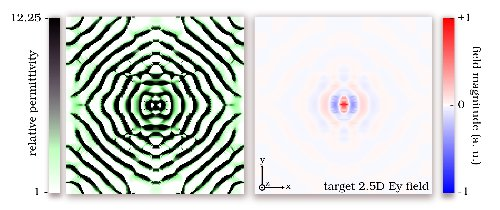
\includegraphics[width=\textwidth]{p2/target}
\caption{The (a) dielectric structure, $\epsilon$, and (b) target field, $E$ ($E_y$ shown only), produced after 75 iterations (10 minutes) on a $160\times 160$ grid. The resulting $\epsilon$ is almost completely binary, and relatively smooth.}\label{target}
\end{figure}
Figs.~\ref{target}a and \ref{target}b are the resulting values of $\epsilon$ and $E$ ($E_y$ shown only), respectively, after 75 iterations of our inverse design method. The entire inverse design process takes only 10 minutes on a standard desktop computer for the $160 \times 160$ grid. An animation of the values of $\epsilon$ and $E_y$ at each iteration of the algorithm is included in the supplementary material.  

The values of the physics residual and the design objective (mode volume) at each iteration are shown in Fig.~\ref{progress}. Most importantly, we see that the physics residual seems to converge linearly, indicating that the algorithm is reasonably efficient. The primary factor in determining this rate of convergence is the exponential decrease in $\eta$ (Eq.~\ref{b1}), since as $\eta$ decreases, increasing emphasis is placed on minimizing the physics residual in the field sub-problem. 

\begin{figure}[hbt]
\centering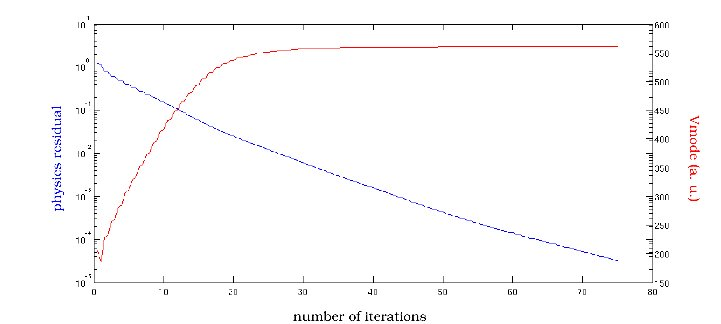
\includegraphics[width=\textwidth]{p2/the_prog}
\caption{Value of the physics residual (blue) and design objective, or mode volume, (red) at each iteration. The physics residual seems to exhibit linear convergence, while the mode volume quickly saturates after roughly 25 iterations.}\label{progress}
\end{figure}

\section{Verification} % Find better section name
\subsection{Accuracy}
To evaluate the accuracy of the inverse design method, we compared the field resulting from the iterations (target field) with the actual field of the resulting structure solved by the 2.5-dimensional approximation (2.5D fiber mode) as well as the field of a full three-dimensional FDTD simulation of the resulting structure (full 3D field), as shown in Figs.~\ref{comp} and \ref{xsec}.

As detailed above, the thickness of the corresponding three-dimensional structure is determined by Eq.~\ref{t}, which yielded a value of $8.16 \Delta x$. However, a small sampling of thicknesses in that vicinity resulted in a more accurate thickness of $8.5\Delta x$, which matched the resonant frequency of the target field and 2.5-dimensional fiber mode.
\begin{figure}[hbt]
\centering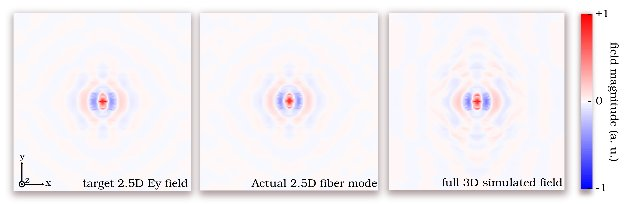
\includegraphics[width=\textwidth]{p2/compare}
\caption{Comparison ($E_y$) of (a) the target field from the inverse design method (from Fig.~\ref{target}), (b) the actual 2.5-dimensional fiber mode, and (c) the field from the full three-dimensional FDTD simulation. The target field matches well with the full three-dimensional field.}\label{comp}
\end{figure}

\begin{figure}[hbt]
\centering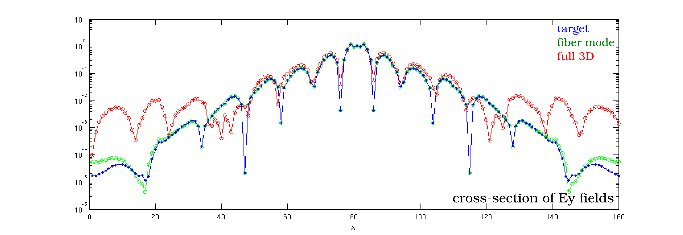
\includegraphics[width=\textwidth]{p2/the_xsec}
\caption{Comparison of the cross sections of the $E_y$ field along the x-axis from the target field (blue), the actual 2.5-dimensional fiber mode (green), and the field from the full three-dimensional FDTD simulation (red). There is some discrepancy between the target field and the full three-dimensional field, but even that is confined to the edges and is only on the order of $\sim 1\%$ of the maximum field amplitude.}\label{xsec}
\end{figure}
Fig.~\ref{comp} plots the $E_y$ component of the target field, 2.5-dimensional fiber mode and the full three-dimensional FDTD field side-by-side. Fig.~\ref{xsec} plots the horizontal cross sections of the magnitudes of the fields on a logarithmic scale. We see that the target field and fiber mode match very well, while there is significantly more discrepancy between the target field and the full three-dimensional field. This is expected with the use of our approximation; however, the error is still relatively small (below 1\% of the maximum field strength) and confined mostly to the edges of the structure.

\subsection{Performance}
The fields from the full three-dimensional FDTD simulation were used to evaluate the performance of the device. The resulting mode volume was $0.32 (\frac{\lambda}{n})^3$ and the total quality factor was 7063. The radiative (out-of-plane) quality factor was 8808 and the in-plane quality factor was 35648.

Fig.~\ref{qcomp} shows the Fourier transforms of the target, fiber and three-dimensional $E_y$ fields taken at the center of the slab. Although there are virtually no field components in the light cone in the case of the target and fiber fields, additional components are present in the full three-dimensional case. This explains why even when leaky radiative components were strictly disallowed in the field optimization sub-problem, the error in the 2.5-dimensional approximation unavoidably introduces some leaky components in the case of the actual three-dimensional structure.

\begin{figure}[hbt]
\centering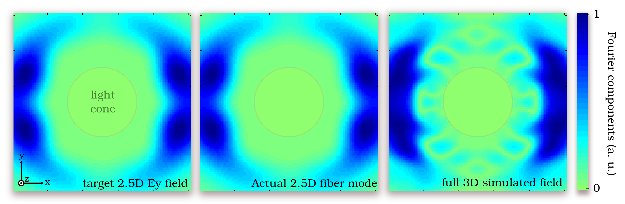
\includegraphics[width=\textwidth]{p2/qcomp}
\caption{Comparison of the Fourier transforms of the $E_y$ fields of the (a) the target field from the inverse design method, (b) the actual 2.5-dimensional fiber mode, and (c) the field from the full three-dimensional FDTD simulation. The error in our approximation introduces some small additional Fourier components into the light cone.}\label{qcomp}
\end{figure}

\section{Conclusion}
In summary, by using a 2.5-dimension approximation, we demonstrate the inverse design of a three-dimensional nanophotonic resonator. Further development of our method includes applying our inverse method to design three-dimensional devices which support multiple fields at different frequencies. This includes resonant devices such as a multi-wavelength cavity, as well as waveguiding devices such as $N$-port couplers, multiplexers, and grating couplers.\\

This work has been supported in part by the AFOSR MURI for Complex and Robust On-chip Nanophotonics (Dr. Gernot Pomrenke), grant number FA9550-09-1-0704.
